\documentclass[conference]{IEEEtran}
\IEEEoverridecommandlockouts
% The preceding line is only needed to identify funding in the first footnote. If that is unneeded, please comment it out.
\usepackage{cite}
\usepackage{amsmath,amssymb,amsfonts}
\usepackage{algorithmic}
\usepackage{graphicx}
\usepackage{textcomp}
\usepackage{xcolor}
\def\BibTeX{{\rm B\kern-.05em{\sc i\kern-.025em b}\kern-.08em
    T\kern-.1667em\lower.7ex\hbox{E}\kern-.125emX}}
\begin{document}

\title{ESE 417 Final Project Classification of Wine Quality by Machine Learning}

\author{\IEEEauthorblockN{1\textsuperscript{st} Haoyu Quan}
\IEEEauthorblockA{\textit{ Mckelvey School of Engineering} \\
\textit{Washington University in St. Louis}\\
St. Louis, MO \\
quanhaoyu@wustl.edu}
\and
\IEEEauthorblockN{2\textsuperscript{nd} Anny Qiao}
\IEEEauthorblockA{\textit{ Mckelvey School of Engineering} \\
\textit{Washington University in St. Louis}\\
St. Louis, MO \\
a.qiao@wustl.edu}
\and
\IEEEauthorblockN{2\textsuperscript{nd} Bruce Li}
\IEEEauthorblockA{\textit{ Mckelvey School of Engineering} \\
\textit{Washington University in St. Louis}\\
St. Louis, MO \\
liyifei@wustl.edu}
}

\maketitle
\section{Introduction}
Machine learning is a branch of artificial intelligence that enables machines to learn from data and make predictions or decisions without being explicitly programmed. It finds applications in a wide range of domains such as image recognition, natural language processing, and predictive modeling. In this project, we aim to use supervised machine learning algorithms to classify a wine quality data set based on 11 given features. While wine was once viewed as a luxury good, it is now enjoyed by a wider range of consumers. Quality evaluation is a crucial part of the certification process and can help to identify influential factors during the wine production process [citation 1]. In our project, these factors will be used as features for our machine learning algorithm.\\

The primary objective of this project is to build a machine learning model that can accurately predict the quality of wine into 10 different levels with the given data. Furthermore, we aim to compare the performance of different machine learning algorithms such as Support Vector Machines (SVM), K-Nearest Neighbors (KNN), and Random Forest to determine the most effective algorithm for this task. To improve the accuracy of our model, we have implemented various methods of data cleaning, chosen optimal weight factors, and tuned other hyperparameters. \\

After multiple testing and trial and error iterations, the model was able to achieve an accuracy rate of over 60 percent. Overall, this project demonstrates the effectiveness of supervised machine learning algorithms in predicting the quality of wine based on various influential factors during the production process.\\

\section{Methods}
\subsection{Exploratory Data Analysis and Cleaning}
\subsection{KNN}
\subsection{Grid Search and Weighted Features}
Grid search is a widely used hyperparameter optimization technique in machine learning that involves systematically evaluating a range of hyperparameters for a given model. This technique entails creating a grid of all possible combinations of hyperparameters and training a model for each combination. The optimal combination of hyperparameters is then determined by selecting the one that yields the highest accuracy or lowest error rate, depending on the specific problem being addressed.\\
In the present project, grid search was employed to fine-tune the hyperparameters of the Support Vector Machine (SVM) model. Specifically, the hyperparameters C and gamma were tuned using grid search to optimize the model's performance. These two hyperparameters are of particular importance in determining the efficacy of the SVM model in handling the data at hand.\\
To accomplish this, a two-stage approach was used, where a broad range of C and gamma values was initially explored, followed by a more focused search of a smaller region to identify the optimal values for these hyperparameters. The implementation of the grid search algorithm used in this project is presented below:
	\begin{figure}[h]
	\label{fig:foo}
	\begin{center}
	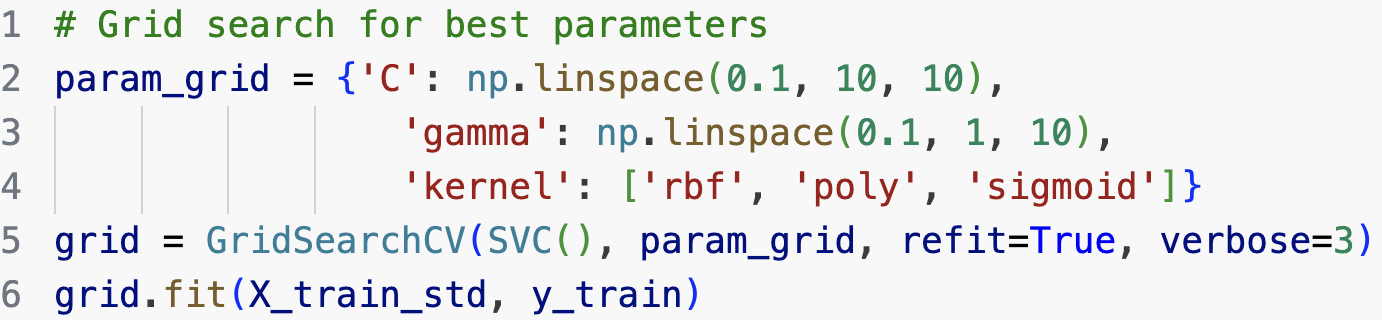
\includegraphics[scale=0.35]{gridSearch.png}
	\caption{Grid Search Code}
	\end{center}
	\end{figure}

\subsection{SVM}
The Support Vector Machine (SVM) is a supervised machine learning algorithm that has gained popularity for its success in various classification tasks, including wine quality classification. SVM works by identifying a decision boundary that effectively separates the different categories of wine quality in the feature space.\\

To classify the wine quality, the SVM requires input features such as alcohol content, acidity, sugar content, and other sensory attributes. The objective of the SVM is to find a hyperplane or a linear decision boundary that can best separate the various quality categories of wine samples in the feature space. The dimensionality of this hyperplane is higher than the dimensionality of the data, and it is determined by selecting a marginal maximization hyperplane. This approach ensures that the SVM classifier is robust by calculating the distance between the hyperplane and the nearest data point for each quality category.\\

However, in cases where the data is not linearly separable, SVMs utilize kernel functions to transform the data to a higher dimensional space, which makes it linearly separable. Among the commonly used kernel functions for wine quality classification are linear, polynomial, radial basis function (RBF), and sigmoid kernels. These kernels map the data into a new feature space, where the SVM can find a hyperplane that separates the different quality categories with a good margin.\\

In this project, SVM has been trained with raw data then with the standardized and cleaned data. Then Grid Search is implemented to find the best hyperparameters of C and gamma. With all the methods implemented with SVM model, the accuracy has a 10$\%$ improvement and MSE has a 33$\%$ decrement. 

\subsection{Random Forest}
Random Forest is an ensemble learning algorithm that is used for classification tasks. It works by constructing multiple decision trees and then combining their predictions to make a final prediction. The algorithm randomly selects a subset of features and a subset of training samples for each decision tree, which helps to reduce overfitting and improve the performance of the model.Also, to simplify the process, the sklearn method of RandomForestClassifier() is used to classify the wine quality. (sklearn). There are eleven features imputed to the ML algorithm. Because the correlation of the wine quality is more related to some features than others, the features need to be considered differently while imputed into the machine learning algorithm. Here are the weights for each feature used in the program :{1: 10, 2: 10, 3: 69, 4: 1, 5: 1, 6: 1, 7: 1, 8: 34, 9: 10, 10: 10, 11: 80.  Those weights are estimated from the input importance of the people originally conducting the experiments.\\
	Due to their great variety of hyperparameters, to optimize the accuracy of the method four are used which are $n estimators, max depth, random state, class weight$. The grid search is implemented to come up with the best combination of the hyperparameters, $ 'max depth': 15, 'n estimators': 700$. With given depth and number of estimators the Machine learning algorithm would output the best performances.\\
	\begin{figure}[h]
	\label{fig:foo}
	\begin{center}
	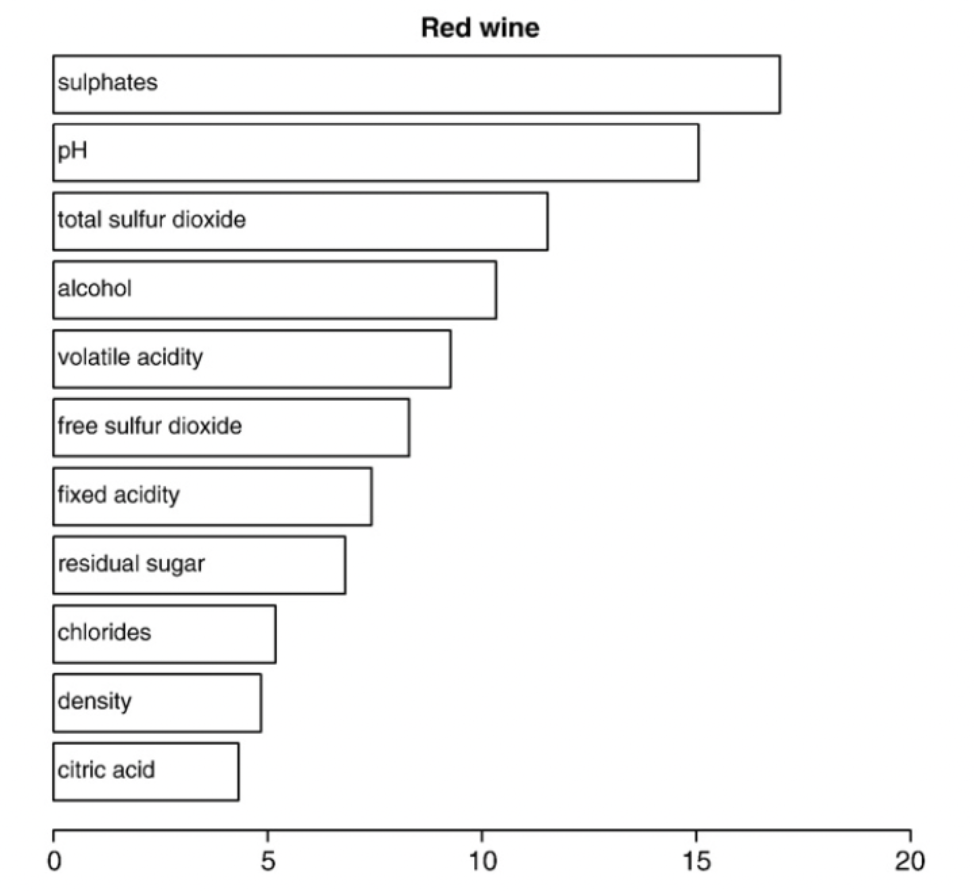
\includegraphics[scale=0.35]{redWineWeight.png}
	\caption{Red Wine Weight}
	\end{center}
	\end{figure}\\
	
\section{Result and Analysis}
Implementing the three method mentioned above shows Random Forest does the best in all the methods. 
\subsection{KNN}
\subsection{SVM}
In the SVM method, no cleaning was performed on the data, and after feeding the data into the SVM model fit, an accuracy of 53$\%$ was obtained. After cleaning the data, the accuracy improved to 63$\%$. The default settings of the parameters of the SVM model were:\\

kernel='rbf', C=1.0, randomstate=0, degree=3, and gamma='auto' \\

A grid search was then performed for the hyperparameters, with C ranging from 0.1 to 10 and gamma ranging from 0.1 to 1, with three types of kernel functions, namely rbf, poly, and sigmoid. The best parameters for the grid search were found to be {'C': 2.3, 'gamma': 0.7, 'kernel': 'rbf'}. The grid search was further refined, with C ranging from 1.8 to 2.8 and gamma ranging from 0.6 to 0.8. The final optimal hyperparameters were determined to be {'C': 2.326, 'gamma': 0.705, 'kernel': 'rbf'}, and the accuracy improved from 63$\%$ to 65.87$\%$.\\
	\begin{figure}[h]
	\label{fig:foo}
	\begin{center}
	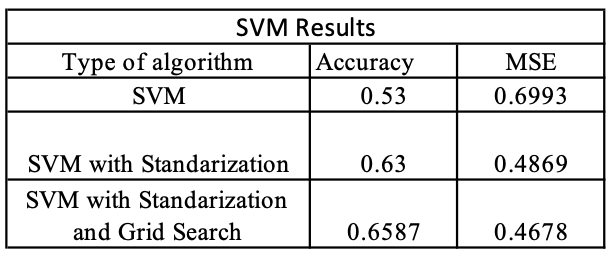
\includegraphics[scale=0.5]{SVMResult.png}
	\caption{SVM Result}
	\end{center}
	\end{figure}\\
With the methods implementation, the MSE is decreasing, which is a good indicator, because 




\subsection{Random Forest}
The grid search parameters demonstrated as following:
	\begin{figure}[h]
	\label{fig:foo}
	\begin{center}
	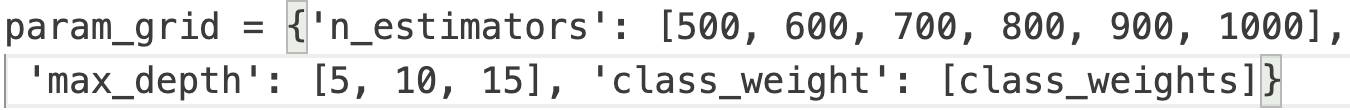
\includegraphics[scale=0.35]{RandomForestGrid.png}
	\caption{Random Forest Grid Search Code}
	\end{center}
	\end{figure}
After trials and errors, the features with the most importance are citric acid and alcohol. The density of the wine still has some weight impact to the wine but not as much. The other variables are not as important. Even the consideration chlorides, free sulfur dioxide and total sulfur dioxide would disrupt the judgment of the algorithm and lower the accuracy of the classification. \\
(1: 10, 2: 10, 3: 69, 4: 1, 5: 1, 6: 1, 7: 1, 8: 34, 9: 10, 10: 10, 11: 80)\\
All method used the random state of 3
	\begin{figure}[h]
	\label{fig:foo}
	\begin{center}
	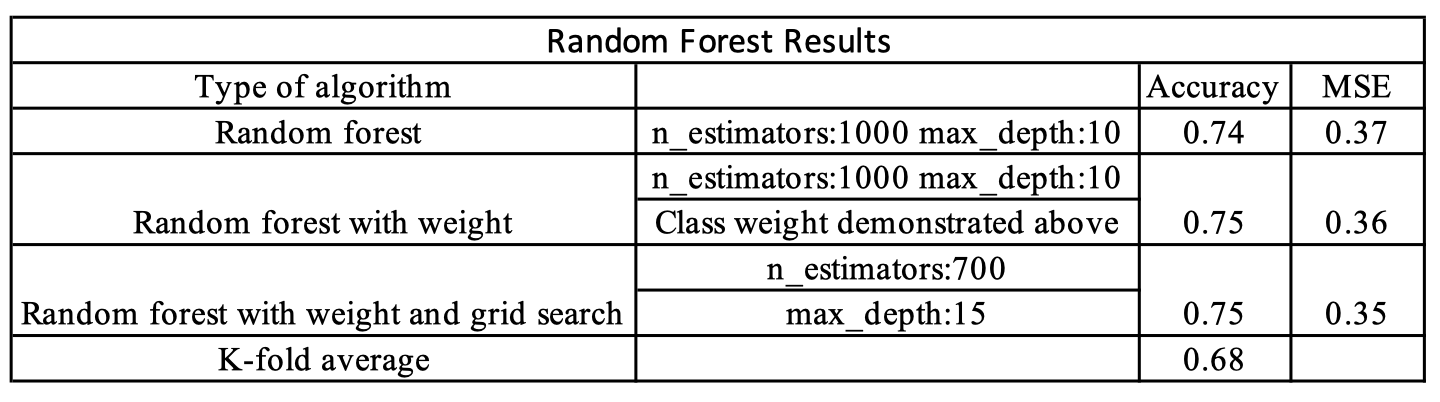
\includegraphics[scale=0.3]{randomForestResult.png}
	\caption{Random Forest Result}
	\end{center}
	\end{figure}





\end{document}
